The algorithm for the two-dimensional FDTD method is derived under the assumption of a TM$^z$ polarization (Transverse Magnetic, the magnetic field is transverse to the direction of propagation $z$). The Faraday and Ampere laws can be written:

\begin{equation}
\begin{cases}
	-\sigma_m\Hvec -\mu \frac{\partial \Hvec}{\partial t} &=
	\nabla \times \Evec	\\
	\sigma \Evec + \epsilon \frac{\partial \Evec}{\partial t} &=
	\nabla \times \Hvec
\end{cases}	
\label{eq:maxwell}
\end{equation}

Using the fact that the only non-zero elements are $E_z$, $H_x$ and $H_y$, (\ref{eq:maxwell}) can be rewritten in the set of scalar equations:

\begin{equation}
	\begin{cases}
		-\sigma_m H_x - \mu\frac{\partial H_x}{\partial t} &=
		\frac{\partial E_z}{\partial y}
		\\
		\sigma_m H_y + \mu\frac{\partial H_y}{\partial t} &=
		\frac{\partial E_z}{\partial x}
		\\
		\sigma E_z + \varepsilon\frac{\partial E_z}{\partial t} &=
		\frac{\partial H_y}{\partial x}
		-\frac{\partial H_x}{\partial y} 
	\end{cases}	
	\label{eq:scalar}
\end{equation}

These equations now need to be discretized in order to be solved numerically. First, the fields are discretized in space and time. $a$ corresponds to the spatial step in the $x$ direction, $b$ to the spatial step in the $y$ direction and $n$ corresponds to the temporal step.

\begin{equation}
    \begin{aligned}
		H_x(x,y,t) &= H_x(a\Delta x, b \Delta y, n \Delta t) \equiv
		H_x^n[a,b]  \\
		H_y(x,y,t) &= H_y(a\Delta x, b \Delta y, n \Delta t) \equiv
		H_y^n[a,b]  \\
		E_z(x,y,t) &= E_z(a\Delta x, b \Delta y, n \Delta t) \equiv
		E_z^n[a,b]
	\end{aligned}
\end{equation}

The derivative of (\ref{eq:scalar}) will then be approximated by finite differences. By neglecting second order terms in the step $\delta$, one can find:

\begin{equation}
	f'(x_0) = \frac{f\left(x_0 + \frac{\delta}{2}\right) - f\left(x_0 - \frac{\delta}{2}\right)}{\delta} + \mathcal{O}(\delta^2) \simeq \frac{f\left(x_0 + \frac{\delta}{2}\right) - f\left(x_0 - \frac{\delta}{2}\right)}{\delta}
	\label{eq:deriv}
\end{equation}

In order to use (\ref{eq:deriv}) to obtain the update equations of the field, it is necessary to include an offset between the electric and magnetic fields. The assumption is done that the electric field nodes are located on integer values of the steps while the magnetic field nodes have offsets of half a step, as shown in Figure \ref{fig:grid}.

\begin{figure}[H]
    \centering
    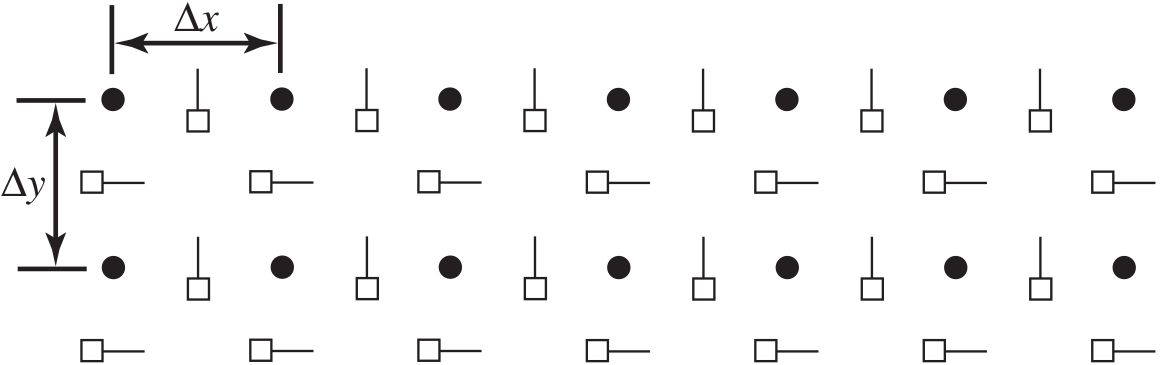
\includegraphics[width=.6\linewidth]{img/grid.png}
    \caption{Physical setup of the FDTD grid. The circles represent the electric field nodes $E$ while the squares represent the magnetic field nodes $H$. An offset of half a spatial step is present\textsuperscript{\ref{fn}}.}
    \label{fig:grid}
\end{figure}

With this particular arrangement of the nodes, the first equation of (\ref{eq:scalar}) can be expanded around the point $(x,y,t) = (a \Delta x, (b+\frac{1}{2}) \Delta y, n \Delta t)$. Each term of the equation is detailed:

\begin{equation}
	\begin{split}
	-\sigma_m H_x^n \left[a,b+\frac{1}{2}\right] &\simeq - \sigma_m \frac{H_x^{n+\frac{1}{2}}\left[a,b+\frac{1}{2}\right] + H_x^{n-\frac{1}{2}}\left[a,b+\frac{1}{2}\right] }{2}\\
	- \mu\frac{\partial H_x}{\partial t} &\simeq - \mu \frac{H_x^{n+\frac{1}{2}}\left[a,b+\frac{1}{2}\right] - H_x^{n-\frac{1}{2}}\left[a,b+\frac{1}{2}\right]}{\Delta t} \\
	\frac{\partial E_z}{\partial y} &\simeq \frac{E_z^{n}\left[a,b+1\right] - E_z^{n}[a,b]}{\Delta y}
	\end{split}
\end{equation}

In the approximated equation, the future term ($H_x$ at time step $n + \frac{1}{2}$) can be obtained from the past ones. Once isolated, it is expressed as: \vspace*{-0.7cm}

\begin{equation}
	H_x^{n+\frac{1}{2}}\left[a,b+\frac{1}{2}\right] =
	\frac{1-\frac{\sigma_m \Delta t}{2 \mu}}{1+\frac{\sigma_m \Delta t}{2 \mu}} H_x^{n-\frac{1}{2}}\left[a,b+\frac{1}{2}\right] -
	\frac{1}{1 + \frac{\sigma_m \Delta t}{2 \mu}} \frac{\Delta t}{\mu \Delta y}
	(E_z^n[a,b+1] - E_z^n[a,b])
	\label{eq:updateHx}
\end{equation}

In (\ref{eq:updateHx}), the parameters $\mu$ and $\sigma_m$ are the value of the material at the space point $(x,y) = (a \Delta x, b + \frac{1}{2} \Delta y)$. Following the same reasoning, the update equations for $H_y$ and $E_z$ can be found:

\begin{equation}
H_y^{n+\frac{1}{2}}\left[a+\frac{1}{2},b\right] =
\frac{1-\frac{\sigma_m \Delta t}{2 \mu}}{1+\frac{\sigma_m \Delta t}{2 \mu}} H_y^{n-\frac{1}{2}}\left[a+\frac{1}{2},b\right] +
\frac{1}{1 + \frac{\sigma_m \Delta t}{2 \mu}} \frac{\Delta t}{\mu \Delta x}
(E_z^n[a+1,b] - E_z^n[a,b])
\end{equation}

\begin{equation}
\begin{aligned}
E_z^{n+1}[a,b] =
\frac{1-\frac{\sigma \Delta t}{2 \epsilon}}{1+\frac{\sigma \Delta t}{2 \epsilon}} E_z^{n}[a,b] + \frac{1}{1+\frac{\sigma \Delta t}{2 \epsilon}}
\left(
\frac{\Delta t}{\epsilon \Delta x} \left\{ H_y^{n+\frac{1}{2} } \left[a + \frac{1}{2}, b\right] -  H_y^{n+\frac{1}{2} } \left[a - \frac{1}{2}, b\right] 
\right\} \right.\\
\left.- \frac{\Delta t}{\epsilon \Delta x} \left\{
H_x^{n+\frac{1}{2} } \left[a,b+ \frac{1}{2}\right] -  H_x^{n+\frac{1}{2} } \left[a, b- \frac{1}{2}\right]
\right\} \right)
\label{eq:update2}
\end{aligned}
\end{equation}